\documentclass[11pt,a4paper]{article}

\usepackage[T1]{fontenc}
\usepackage[utf8]{inputenc}
\usepackage{lmodern}
\usepackage[margin=2.5cm,headheight=14pt]{geometry}
\usepackage{microtype}
\usepackage{amsmath,amssymb}
\usepackage{graphicx}
\usepackage{booktabs,tabularx,array}
\usepackage[font=small,labelfont=bf,labelsep=period]{caption}
\usepackage{xcolor}
\usepackage[authoryear,round]{natbib}
\usepackage{fancyhdr}
\usepackage[hidelinks]{hyperref}
\hypersetup{colorlinks=true,linkcolor=accent,citecolor=accent,urlcolor=accent,
  pdftitle={Can We Sing a Rainbow?},pdfauthor={Derek Reid}}

\definecolor{accent}{RGB}{31,95,191}
\newcommand{\sh}{\ensuremath{\sharp}}
\newcommand{\dg}{\ensuremath{^\circ}}
\newcolumntype{L}{>{\raggedright\arraybackslash}X}
\renewcommand{\arraystretch}{1.15}
\setlength{\parskip}{0.35\baselineskip}
\setlength{\parindent}{0pt}
\bibliographystyle{plainnat}

\pagestyle{fancy}
\fancyhf{}
\fancyhead[L]{\small\itshape Can We Sing a Rainbow?}
\fancyhead[R]{\small\itshape D.~Reid}
\fancyfoot[C]{\small\thepage}
\renewcommand{\headrulewidth}{0.4pt}

\begin{document}

\thispagestyle{plain}
\begin{center}
  {\LARGE\bfseries Can We Sing a Rainbow?\par}
  \vspace{0.4em}
  {\large On the Absence of Radio Rainbows and the Sonification of the Optical One\par}
  \vspace{1.2em}
  {\large Derek Reid\par}
  \vspace{0.3em}
  {\small October 2026\par}
\end{center}
\vspace{0.5em}

\begin{abstract}
\noindent The children's song exhorts us to ``sing a rainbow'', but the physics of doing so has received surprisingly little attention. We first ask whether rainbows emit, or could be detected at, radio frequencies. A rainbow is not a source but a caustic: sunlight refracted and internally reflected by raindrops into a cone of half-angle about 42\dg\ around the antisolar point, unique to each observer. The mechanism needs droplets much larger than the wavelength. For radio waves on millimetre-scale raindrops, scattering is Rayleigh-like and featureless; at sub-millimetre wavelengths, where the sizes become comparable, absorption by water suppresses the internal ray paths. We therefore predict, with some confidence and mild disappointment, that there are no natural radio rainbows.

We then propose a large dielectric prism illuminated by the Sun and by artificial lamps. Solar microwave emission should be measurably refracted but negligibly dispersed, while the radio emission of lamps comes from their drive electronics, not their light. Finally we turn to the optical bow. Transposing the visible spectrum (430--750\,THz) down by 40 octaves maps it to roughly G4--F5, a span of about a minor seventh. Using synthesised audio from model spectra, we show that a continuous source such as sunlight sounds like band-limited noise, and a scan across the bow sounds like a filter sweeping open from the low end. Line-spectrum sources fare better: a fluorescent tube produces a recognisable whole-tone chord. We describe simple experiments with fluorescent tubes that let the reader hear this for themselves. We conclude that one can indeed sing a rainbow, provided one is content to hum.

\medskip
\noindent\textbf{Keywords:} rainbow; Mie scattering; microwave refraction; sonification; spectral lines; fluorescent lamps
\end{abstract}

%-------------------------------------------------------------------------
\section{Introduction}

We can sing a rainbow, but only after lowering it by 40 octaves, and it mostly hums. This paper explains why, and why no radio telescope will do it for us.

The song ``I Can Sing a Rainbow'' \citep{hamilton1955} lists the colours red, yellow, pink, green, purple, orange and blue, and invites the listener to sing them. Taken literally, this raises three questions:
\begin{enumerate}
  \item Does a rainbow emit anything outside the visible band, in particular radio waves that a receiver could turn into sound?
  \item If not, can we build an artificial rainbow, a large prism, that spreads radio waves the way a rainbow spreads light?
  \item Failing both, what would the visible rainbow sound like if we simply moved its frequencies down into the range of hearing?
\end{enumerate}

A rainbow is not an object. Sunlight enters a spherical raindrop, refracts, reflects once off the back surface and refracts out again. Light leaving the drop piles up near a minimum deviation angle of about 138\dg, so it returns about 42\dg\ from the antisolar point \citep{descartes1637}; for modern accounts see \citet{nussenzveig1977}, \citet{lee2001} and \citet{adam2002}. Because the refractive index of water falls slightly from violet to red, each colour has its own angle, and the bow is spread from about 40.5\dg\ (violet) to 42.4\dg\ (red). Every observer sees a different set of drops, so there is no single rainbow to point an antenna at.

Rainbows and sound have met before, in three different senses. True acoustic rainbows, caustics just like the optical one, appear when sound scatters from fluid spheres in which it travels more slowly than in the surrounding water \citep{marston1983}. Acoustic ``rainbow trapping'' metamaterials \citep{zhu2013} and topology-optimised acoustic prisms \citep{christiansen2025} sort broadband sound by frequency into different positions or directions: rainbows in the colour-sorting sense, not the 42\dg\ sense. This paper asks the reverse question: not how to make a rainbow out of sound, but how to make sound out of a rainbow.

%-------------------------------------------------------------------------
\section{Why there are no radio rainbows}

A rainbow needs drops much larger than the wavelength, and at radio wavelengths raindrops are hundreds to thousands of times too small. The relevant number is the size parameter, the drop's circumference divided by the wavelength,
\begin{equation}
  x = \frac{2\pi a}{\lambda},
\end{equation}
where $a$ is the drop radius. The geometric-optics rainbow of Section~1 is accurate for $x$ of several hundred or more. Supernumerary bows and Airy's wave correction \citep{airy1838} appear as $x$ falls into the tens to low thousands. Below $x\approx1$ there is no ray path at all: the drop scatters as a tiny dipole (Rayleigh scattering), with intensity falling as the fourth power of wavelength and no preferred angle near 42\dg\ (Table~\ref{tab:regimes}).

\begin{table}[ht]
\centering
\caption{Size parameter of a 1\,mm raindrop across the spectrum, and whether a bow can form.}
\label{tab:regimes}
\small
\begin{tabularx}{\linewidth}{@{}l l r l L@{}}
\toprule
Band & Wavelength & $x$ & Regime & Rainbow? \\
\midrule
Visible light & 0.4--0.7\,\textmu m & 9{,}000--16{,}000 & Geometric optics & Yes \\
Far infrared / THz & 0.1--1\,mm & 6--60 & Mie resonances & No: water absorbs the internal ray within ${\sim}0.1$\,mm \\
Millimetre wave (100\,GHz) & 3\,mm & 2 & Mie & No \\
Weather radar (3\,GHz) & 10\,cm & 0.06 & Rayleigh & No \\
FM radio (100\,MHz) & 3\,m & 0.002 & Rayleigh & No \\
\bottomrule
\end{tabularx}
\end{table}

The one band where the sizes almost match, the far infrared, is closed by water itself. Liquid water absorbs so strongly there that light entering a drop is gone long before it reaches the back surface to reflect. With no internal reflection, there is no bow.

Rain does interact with radio, and usefully: weather radar measures exactly this Rayleigh scattering \citep{noaanws}, whose strength scales with the sixth power of drop diameter. But radar echoes come back in all directions, with no bright 42\dg\ cone. A radio rainbow would need drops about a metre across, which is not a form of weather we would wish on anyone.

%-------------------------------------------------------------------------
\section{The giant prism: sunlight versus lamps at radio frequencies}

A metre-scale prism of the right material will bend the Sun's microwaves by tens of degrees but will barely spread them into a spectrum, and it does nothing at all to the radio noise from lamps. If nature won't make a radio rainbow, we can try to build one. A prism avoids the size problem of Section~2: we can make it as large as we like.

\subsection{The source: the Sun is a radio transmitter}

The Sun is bright at centimetre wavelengths, with a brightness temperature of order 10{,}000\,K at 10--12\,GHz. That is easily detected with a domestic satellite dish, Ku-band LNB and satellite-finder meter or software-defined radio; a commercial satellite-TV dish has been used to measure the Sun's flux at 11.2\,GHz \citep{mandal2016}. Daily 10.7\,cm solar flux (the F10.7 index) has been a standard space-weather measurement since 1947 \citep{noaaswpc}.

\subsection{The experiment}

\begin{enumerate}
  \item Mount a satellite dish (about 80\,cm) with a Ku-band LNB (10.7--12.75\,GHz) on a steerable mount, and log signal strength.
  \item Map the Sun with no prism: a drift scan gives its position and the dish's beam width (about 2\dg\ at 11.7\,GHz for an 80\,cm dish).
  \item Place a 60\dg\ prism across the dish aperture. It must be at least as large as the dish, which is why the prism needs faces of a metre or more.
  \item Map the Sun again. The peak should move by the prism's deviation angle.
  \item Repeat at the band's two ends (10.7 and 12.75\,GHz) to look for dispersion: a shift of peak position between them.
\end{enumerate}

\subsection{What to build it from}

The deviation at minimum deviation, for apex angle $A$ and refractive index $n$, is
\begin{equation}
  D = 2\arcsin\!\left(n\sin\frac{A}{2}\right) - A .
\end{equation}
The material matters more than the size: it must be transparent at 12\,GHz, not just in visible light (Table~\ref{tab:materials}).

\begin{table}[ht]
\centering
\caption{Candidate prism materials at about 12\,GHz. Deviations are for a 60\dg\ prism at minimum deviation.}
\label{tab:materials}
\small
\begin{tabularx}{\linewidth}{@{}l c c c L@{}}
\toprule
Material & $n$ & Loss & Deviation & Verdict \\
\midrule
PTFE (Teflon) & 1.44 & ${\sim}0.3$\,dB/m & ${\sim}32\dg$ & Ideal, but about a tonne and costly \\
Paraffin (candle) wax & 1.5 & $<1$\,dB/m & ${\sim}37\dg$ & Best value; the classic teaching-lab microwave prism \citep{umd} \\
Solid perspex (PMMA) & 1.6 & ${\sim}9$\,dB/m & ${\sim}46\dg$ & Works, with some loss \\
Window glass & ${\sim}2.4$ & 10--20\,dB/m & none & Total internal reflection ($n>2$); also too lossy and several tonnes \\
Perspex shell filled with water & ${\sim}8$ & ${\sim}3$\,dB/mm & --- & Acts as a mirror (Section~3.4) \\
\bottomrule
\end{tabularx}
\end{table}

The expected result is clear refraction with almost no dispersion. PTFE and wax have almost no change in refractive index across 10--13\,GHz, so the two ends of the band leave the prism within a small fraction of a degree of each other, well inside the dish's 2\dg\ beam. We would have bent a radio beam, but not made a radio rainbow.

\subsection{The water-filled perspex prism}

A hollow perspex prism filled with water behaves completely differently in the two bands, and both results are worth having.

\textbf{In visible light it is the best prism of all for this paper.} The flat, parallel perspex walls add no net deviation, so the light is bent by the water alone. Water's refractive index (about 1.333) gives a minimum deviation of about 24\dg, and red to violet spread over about 1\dg, roughly 9\,cm on a screen 5\,m away. This is a rainbow made from rainbow material: the same water, with the same dispersion, that makes the real bow. A solid perspex prism ($n\approx1.49$) bends light more (about 36\dg) and spreads it a little wider (about 1.5\dg). Mind the weight: an equilateral prism 2\,m on a side and 2\,m deep holds about 3.5 tonnes of water, and the bottom panel takes about 20\,kPa of pressure. A 30\,cm version works just as well optically.

\textbf{At microwave frequencies it is a mirror.} Water at 10--12\,GHz has a refractive index of about 8 and is extremely absorbing: microwaves lose about 3\,dB per millimetre, which is why microwave ovens work. About 60\% of the Sun's signal would reflect off the first face and the rest would be absorbed within a few millimetres. Ironically, water is strongly dispersive at microwaves (its molecular relaxation peak is near 20\,GHz), but, as with raindrops in the far infrared, the absorption hides it. At VHF (100\,MHz) tap water is less lossy, and its index of about 9 makes total internal reflection catch everything: the critical angle is about 6\dg, so no ray could leave the second face of a 60\dg\ prism. A water prism is excellent for light and useless for radio.

\subsection{Artificial lamps}

Lamps make a useful control, because their radio output has nothing to do with their light. An incandescent filament is far smaller than a centimetre wavelength and is a poor (metallic) thermal emitter, so its thermal radio emission is undetectable beside the Sun. LEDs emit no measurable thermal radio at all. What a receiver near a lamp does pick up is electronic interference, from LED drivers, fluorescent ballasts and dimmers, at kHz to MHz frequencies. Those wavelengths are metres to kilometres, so a 2\,m prism has no effect on them. The comparison is therefore: the Sun's radio passes through the prism and is bent; the lamps' ``radio'' never came from the light in the first place.

%-------------------------------------------------------------------------
\section{Sonifying the optical rainbow}

We hear light by dividing every optical frequency by $2^{40}$, which lowers it exactly 40 octaves and lands the whole visible spectrum between about F\sh4 and F5. Since a radio receiver cannot help us, we take the visible rainbow itself and move it into the audible range:
\begin{equation}
  f_{\mathrm{audio}} = \frac{c}{\lambda\,2^{40}} .
\end{equation}
Dividing by a power of two keeps every musical interval intact: two spectral lines a fifth apart in optical frequency are still a fifth apart in sound. Newton drew the same analogy in reverse, dividing the spectrum ``after the manner of a Musical Chord'' \citep{newton1730}. Colour organs that play light like music go back to the eighteenth century \citep{peacock1988}, and sonification is now an established tool in astronomy \citep{zanella2022,chandra2020}. Unlike Newton's division, ours has no free choices: the mapping is fixed by physics and one integer (Table~\ref{tab:notes}).

\begin{table}[ht]
\centering
\caption{The visible spectrum transposed down 40 octaves.}
\label{tab:notes}
\small
\begin{tabular}{@{}r l r l@{}}
\toprule
Wavelength & Colour & Audio frequency & Nearest note \\
\midrule
750\,nm & Deep red (limit of vision) & 364\,Hz & F\sh4 \\
700\,nm & Red & 390\,Hz & G4 \\
650\,nm & Red & 420\,Hz & G\sh4 \\
605\,nm & Orange & 451\,Hz & A4 (sharp) \\
580\,nm & Yellow & 470\,Hz & A\sh4 \\
530\,nm & Green & 515\,Hz & C5 (flat) \\
470\,nm & Blue & 580\,Hz & D5 \\
430\,nm & Violet-blue & 634\,Hz & D\sh5 \\
400\,nm & Violet & 682\,Hz & F5 (flat) \\
\bottomrule
\end{tabular}
\end{table}

The whole of human vision fits in a little under an octave, from 750\,nm to 400\,nm, a frequency ratio of 1.875. The ear hears about ten octaves; the eye sees less than one. The rainbow is a very short song.

\paragraph{Synthesis.} Each clip is synthesised from a model spectrum, not recorded from a real instrument; Section~6 describes how to measure the real ones.
\begin{itemize}
  \item Continuous spectra (the Sun, a filament, an LED's phosphor) become shaped noise. We build the sound's spectrum directly: each audio frequency gets the amplitude of the light at its corresponding wavelength, with random phase, and an inverse Fourier transform gives the waveform. This is the correct sound of incoherent thermal light, which has random phases.
  \item Spectral lines (mercury, sodium, hydrogen, neon, the rare-earth phosphors in fluorescent tubes) become near-pure tones at their transposed frequencies, with relative loudness set by their relative power.
  \item The Sun uses a 5778\,K blackbody with the strongest Fraunhofer absorption lines cut in. The incandescent lamp uses 2700\,K.
  \item The rainbow scan uses Airy's theory \citep{airy1838} for each of 90 wavelengths, with 0.25\,mm drops, smeared by the Sun's 0.53\dg\ disc. Water's refractive index follows a Cauchy fit (1.3435 at 404\,nm, 1.3308 at 706\,nm), placing the primary bow between 40.5\dg\ (violet) and 42.4\dg\ (red).
  \item All clips are normalised to the same loudness ($-20$\,dBFS RMS), 8\,s long, 44.1\,kHz mono. We do not weight by the eye's sensitivity, so a clip sounds like the light's physical spectrum, not its perceived colour.
\end{itemize}

%-------------------------------------------------------------------------
\section{Results: what light sounds like}

Smooth spectra hiss and line spectra play chords (Figure~\ref{fig:sources}). Sunlight and lamps with continuous spectra sound like wind through a narrow filter, while gas-discharge lamps produce recognisable notes, and the fluorescent tube plays a whole-tone chord. Table~\ref{tab:clips} describes each clip.

\begin{figure}[ht]
  \centering
  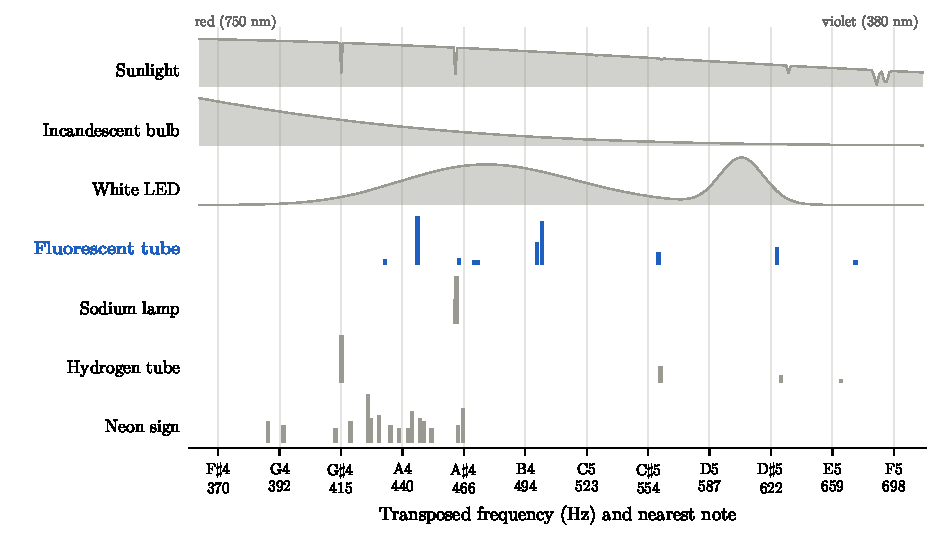
\includegraphics[width=\linewidth]{fig_sources.pdf}
  \caption{Model spectra of seven light sources, transposed down 40 octaves onto a musical axis. Continuous sources (grey areas) are heard as hiss; line sources (bars) are heard as notes. The fluorescent tube (blue) lands on A4, B4, C\sh5 and D\sh5, each about 20 cents sharp. Heights are relative power within each source.}
  \label{fig:sources}
\end{figure}

\begin{table}[ht]
\centering
\caption{The ten supplementary audio clips. Files are named \texttt{NN\_description.wav}.}
\label{tab:clips}
\small
\begin{tabularx}{\linewidth}{@{}r l L@{}}
\toprule
Clip & Source & What you hear \\
\midrule
01 & Sunlight (5778\,K) & Band-limited hiss from about 364 to 718\,Hz, centred near 507\,Hz. Like wind, or a distant waterfall. \\
02 & Filament bulb (2700\,K) & The same hiss tilted downward, centred near 434\,Hz. Audibly darker: the bulb's ``warm white'' is a warm hiss. \\
03 & White LED & A whistle near 606\,Hz (the 450\,nm blue chip) over a broad hiss (the yellow phosphor). \\
04 & Triphosphor fluorescent tube & A chord: A4, B4, C\sh5 and D\sh5, each about 20 cents sharp, with faint A\sh4 and E5. A whole-tone cluster over a soft hiss. \\
05 & Low-pressure sodium lamp & A single note, A\sh4 at 463\,Hz, that swells and fades about every two seconds. \\
06 & Hydrogen discharge tube & G\sh4, C\sh5, D\sh5 and E5: a C\sh\ minor chord with an added ninth. \\
07 & Neon sign & Sixteen lines packed between G4 and A\sh4. A dense, beating tone cluster, like a swarm of bees. \\
08 & A scan across the rainbow & Silence, then a low hiss that brightens from the bottom up, then a steady full-band hiss. \\
09 & The song's seven colours & G\sh4, A\sh4, G\sh4 with hiss, C5, G\sh4\,+\,D\sh5, A4, D5. \\
10 & Fluorescent tube via a photodiode & A 100\,Hz mains buzz. Not transposed: what a real tube sounds like through a solar cell (Section~6). \\
\bottomrule
\end{tabularx}
\end{table}

\paragraph{The sunlight hiss is not quite featureless, but it sounds so.} The Fraunhofer absorption lines are real gaps in the spectrum (visible as notches in Figure~\ref{fig:sources}). But they are only about 0.1\,nm wide, which becomes about 0.1\,Hz in audio, far too narrow for the ear to notice in noise. To hear them they would have to be widened about a hundredfold.

\paragraph{The sodium lamp beats.} Its two D lines, at 588.995 and 589.592\,nm \citep{nist}, transpose to 462.9 and 462.5\,Hz. Two tones that close beat against each other at their difference, 0.47\,Hz. The lamp plays one note that pulses slowly, like a singer breathing. This is the sodium doublet made audible: a fine-structure splitting caused by electron spin, heard as a tremolo.

\paragraph{The rainbow scan fills from the bottom.} Outside the primary bow lies Alexander's dark band, which is silent (Figure~\ref{fig:scan}). Moving inward, red appears first at 42.4\dg, so the sound begins as a low hiss around G4. As each shorter wavelength joins (violet last, at 40.5\dg), the upper edge of the hiss climbs, like a synthesiser filter opening. The sound's centre of mass rises from about 410 to 560\,Hz over the bow's 2\dg, then settles into the steady full-spectrum hiss of the bright sky inside the bow, gently swelling with the supernumerary arcs. Because no colour switches off as you move inward, a rainbow is not a glissando but a crescendo of brightness from the bass upward.

\begin{figure}[ht]
  \centering
  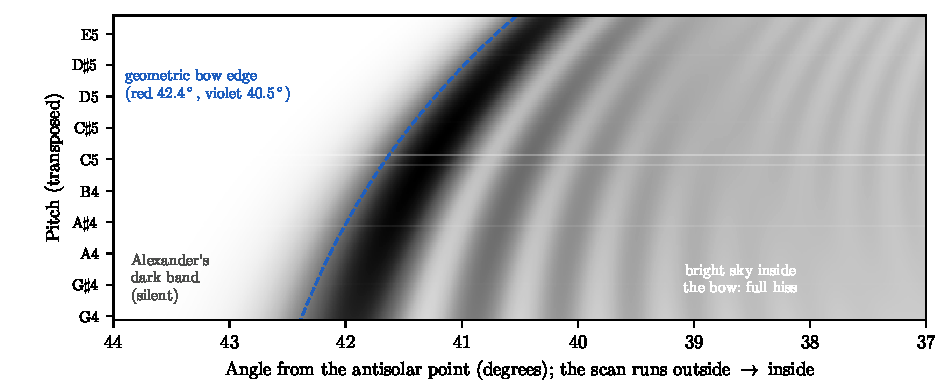
\includegraphics[width=\linewidth]{fig_scan.pdf}
  \caption{Brightness of the primary bow (Airy theory, 0.25\,mm drops, smeared by the solar disc) against scattering angle and transposed pitch. Reading left to right is clip~08: silence, a dark band that fills from the low notes upward, then the supernumerary arcs. The dashed line is the geometric-optics edge. Faint horizontal lines are solar Fraunhofer lines.}
  \label{fig:scan}
\end{figure}

\paragraph{Singing the song.} The song's colours are red, yellow, pink, green, purple, orange and blue. Two are not in the rainbow at all. Pink is a desaturated red (red plus white), so it sounds as G\sh4 under a wash of hiss. Purple is red plus blue, which no single wavelength can make, so it sounds as two notes at once, G\sh4 and D\sh5, a perfect fifth. The resulting ``melody'' is G\sh, A\sh, G\sh, C, G\sh+D\sh, A, D. It is not Arthur Hamilton's tune, and we do not recommend it to choirs.

%-------------------------------------------------------------------------
\section{Fluorescent tubes: experiments to try}

Fluorescent tubes are the most musical light source in the home, and two cheap experiments let you hear them: one through their spectrum, one directly. Both use equipment costing a few pounds.

\subsection{Hear the chord: measure the spectrum}

\begin{enumerate}
  \item Make a spectroscope from a cereal box, a narrow slit and a piece of CD or DVD as a diffraction grating, or buy a pocket spectroscope.
  \item Look at a fluorescent tube. Instead of a smooth rainbow you will see a handful of sharp coloured lines: violet and blue mercury lines, a bright green line, and a strong orange-red line from the europium phosphor.
  \item Photograph the spectrum with a phone held against the eyepiece. Calibrate the wavelength scale using two known lines: mercury green at 546.1\,nm and mercury blue at 435.8\,nm.
  \item Read the brightness along the spectrum and replace the model spectrum in the accompanying generator with your measurement. You will hear your own lamp's chord.
\end{enumerate}

\subsection{Compare tubes, and see whether the chord changes}

\begin{itemize}
  \item \textbf{Warm white, cool white and daylight tubes} use the same three phosphors in different proportions. Prediction: the same notes, with a different balance (warm white louder at A4, daylight louder at C\sh5 and D\sh5). The chord's voicing changes, not its notes.
  \item \textbf{Old halophosphate tubes} (common before the 1990s) have broad emission bands, not sharp lines. Prediction: much more hiss and a far weaker chord.
  \item \textbf{Warm-up.} Record the spectrum every 30 seconds after switching on a cold tube. Does the chord's balance shift as the mercury vapour pressure rises? We have not tested this, and would like to know.
  \item \textbf{Sodium street lamp} (low-pressure, the old deep-orange kind). One note, beating slowly (Section~5). The modern white LED street lamps that replaced them play the LED's whistle-over-hiss instead.
\end{itemize}

\subsection{Listen to light directly with a solar cell}

This experiment involves no transposition: you hear the light's flicker as it really is. It is a standard school practical \citep{iop}.
\begin{enumerate}
  \item Take a small solar cell (from a garden light) or a photodiode and solder it to a 3.5\,mm jack.
  \item Plug it into an amplified computer speaker, or a computer's line or microphone input with recording software.
  \item Point it at different light sources (Table~\ref{tab:flicker}).
\end{enumerate}

\begin{table}[ht]
\centering
\caption{What a solar cell connected to an amplifier hears from different light sources.}
\label{tab:flicker}
\small
\begin{tabularx}{\linewidth}{@{}l L@{}}
\toprule
Light source & Expected sound \\
\midrule
Sunlight & Silence. Sunlight does not flicker, apart from slow changes as clouds pass. \\
Incandescent bulb & A soft 100\,Hz hum. The filament cools slightly between each mains half-cycle, but its heat smooths most of the flicker. \\
Fluorescent tube, magnetic ballast & A loud, buzzy 100\,Hz tone with strong harmonics (clip~10). Light output swings by 43--49\% at 100\,Hz \citep{wilkins1989}. \\
Fluorescent tube or CFL, electronic ballast & Nearly silent. The flicker is at 20--60\,kHz, above hearing; a bat detector will make it audible. \\
LED bulb & Anything from silence (good driver) to a loud 100\,Hz buzz (cheap driver). This doubles as a quality test. \\
TV remote control & Clicks and chirps from its 38\,kHz-modulated infrared bursts. \\
\bottomrule
\end{tabularx}
\end{table}

In 50\,Hz countries such as the UK, flicker is at 100\,Hz because the light peaks on both halves of each mains cycle (120\,Hz in 60\,Hz countries). This experiment is the real-world answer to the sunlight-versus-lamps question of Section~3: the Sun is silent, and every lamp betrays its power supply.

\subsection{Safety}

\begin{itemize}
  \item Never connect anything to the lamp's wiring. The solar cell only needs to see the light.
  \item Don't break fluorescent tubes or CFLs: they contain mercury. Dispose of them at a recycling point.
  \item Never look at the Sun, even through a spectroscope. Point the spectroscope at a white card lit by sunlight, or at blue sky.
\end{itemize}

%-------------------------------------------------------------------------
\section{Discussion and conclusion}

There are no radio rainbows, a radio prism bends without spreading, and the optical rainbow, lowered 40 octaves, hums a soft hiss a little under an octave wide. The song's request can be met only in part.

\paragraph{What we can and cannot claim.} The physics of Sections~2 and~3 is standard and the numbers are robust to an order of magnitude. The sounds of Section~5 are faithful to their model spectra, but they are syntheses, not recordings: a measured spectrum (Section~6.1) would differ in detail, especially in the relative loudness of lines. The 40-octave transposition is a choice, though a natural one, since it is the power-of-two shift that places the visible band in the range of the singing voice. (Three octaves fewer, 37, would put it at 2.9--5.7\,kHz, where the ear is most sensitive, but no one could sing it.)

\paragraph{Three lessons.}
\begin{enumerate}
  \item \emph{Size decides everything.} Whether a drop makes a rainbow depends on its size relative to the wavelength, and at radio wavelengths raindrops are hopelessly small.
  \item \emph{Absorption hides dispersion.} Water is strongly dispersive in both the far infrared and the microwave, but in both bands it absorbs too strongly for a bow or a prism spectrum to form.
  \item \emph{Smooth spectra hiss; line spectra sing.} A continuous source like the Sun has nothing to sing but noise. Atoms, with their discrete energy levels, are the ones that play notes, and the humble fluorescent tube is a four-note instrument hanging from most office ceilings.
\end{enumerate}

\paragraph{Further work.} The most satisfying follow-up would be the dish-and-prism experiment of Section~3.2, since bending the Sun's microwaves with a block of candle wax is a striking result for a modest outlay. Recording real fluorescent spectra across tube types (Section~6.2) would test our predictions about chord voicing. And a choir willing to sing G\sh, A\sh, G\sh, C, G\sh+D\sh, A, D in public would settle, at last, whether one can truly sing a rainbow.

We conclude that one can, provided one is content to hum.

\section*{Supplementary material}
Ten audio clips (WAV, 8\,s, 44.1\,kHz) and the Python generator used to synthesise them and to draw Figures~\ref{fig:sources} and~\ref{fig:scan} accompany this paper.

\bibliography{refs}

\end{document}
